\hypertarget{MK}{\section{Mock-up Interfaces}}
We think that the success or the failure of one application strongly depends on his user-friendly graphic design. According to this we propose, both in the RASD and in the DD documents, some mockups trying to be as intuitive and satisfactory as possible.\\
We also want to offer the possibility to run the two applications on a large number of devices. 
In order to facilitate the diffusion of the Data4Help and AutomatedSOS applications, we want that they run properly on different hardware platforms: personal computer, mobile phone and also wearable devices. In the RASD document we have already presented some UI that accomplish this multi-platform requirement.
Moreover, we designed our application with the purpose to be resizable, so that it can adapt to screens of different dimension.\\
In the RASD document are illustrated 12 different mockups that represent different parts of Data4Help and AutomatedSOS applications. Here we want to introduce 4 new mockups, to increment and complete the overview of the graphic appearance of the two applications. \\
In particular, in this document, we focused on:
\begin{itemize}
    \item \textbf{Menu:}
    From this page, the user can reach all the pages of Data4Help application by clicking on the respective item.
    \item \textbf{Home page:}
    Here the user can see his real-time position on a map(based on Google Maps) and his real-time health parameters.
    Moreover he/she can see the notification for the new requests.
    \item \textbf{Manage requests:}
    In this page the user can accept or decline the requests for his/her data and he/she can interrupt the subscriptions to updated data previously accepted.
    \item \textbf{History:}
    By selecting a time interval, the user can see the average of the value of his/her health parameters and he/she can also observe his historic route.
\end{itemize}
\clearpage
\begin{figure}[ht]
    \centering
    \begin{subfigure}[t]{0.38\linewidth}
        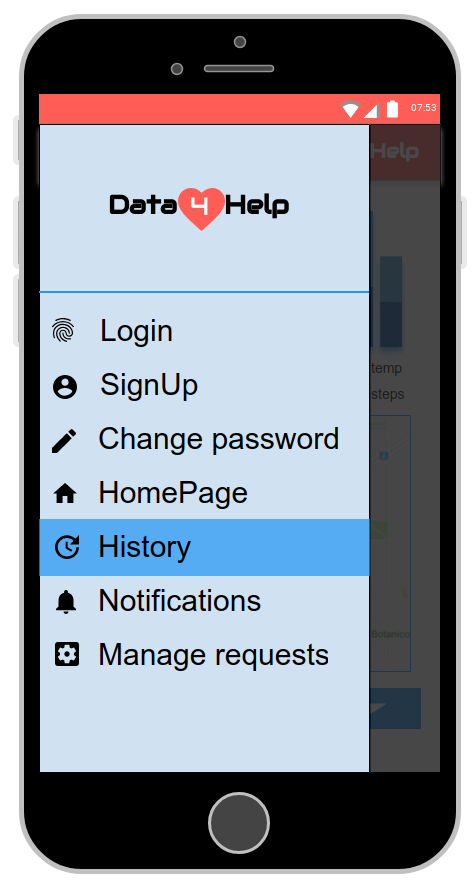
\includegraphics[width=\linewidth]{images/Mockup/Menu.png}
        \caption{Data4Help menu.}
    \end{subfigure} \hfil \hfil \hfil
    \begin{subfigure}[t]{0.38\linewidth}
        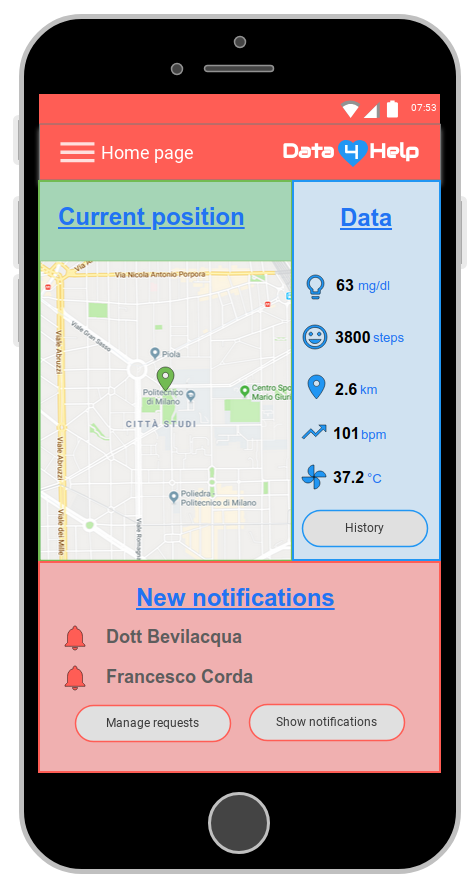
\includegraphics[width=\linewidth]{images/Mockup/Home_page.png}
        \caption{Data4Help Home page.}
    \end{subfigure}
    
  \begin{subfigure}[t]{0.38\linewidth}
    \centering
    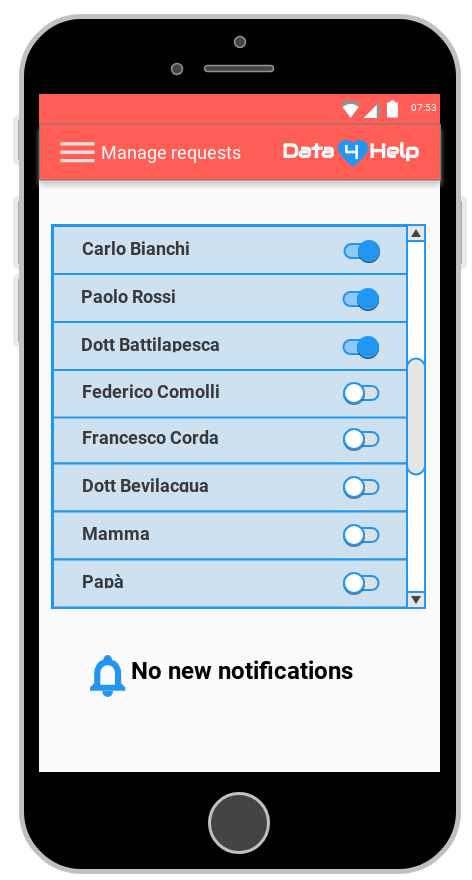
\includegraphics[width=\linewidth]{images/Mockup/Manage_requests.png}
    \caption{User manages his requests.}
  \end{subfigure} \hfil \hfil \hfil
  \begin{subfigure}[t]{0.38\linewidth}
    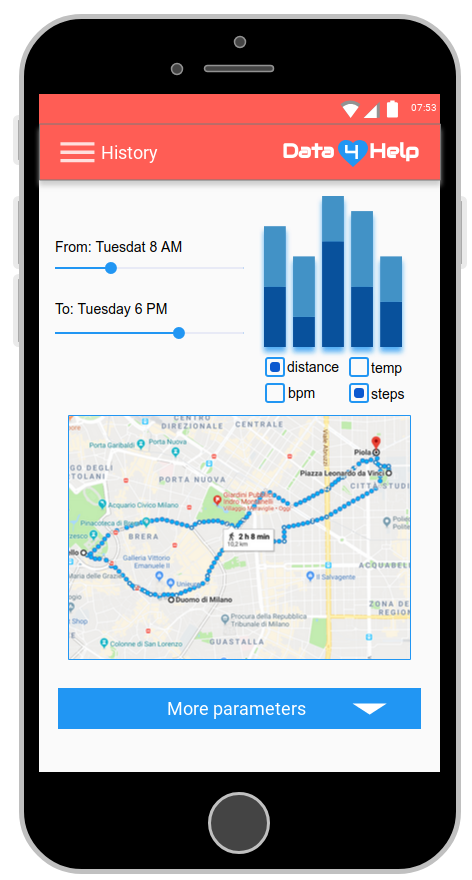
\includegraphics[width=\linewidth]{images/Mockup/History.png}
    \caption{User can observe his historical data.}
  \end{subfigure}
\end{figure}
\clearpage

\section{User Experience Diagrams}
We have already presented how the different screens of our application will look like, showing some comprehensive mockups in the \hyperlink{MK}{\underline{section just above}} and in the RASD document. However they are in some way \say{static}, and just by observing all the presented interfaces it's not possible to understand how they interact with each other.
To this purpose, here are presented three different User Experience diagrams with the intention to cover all the possible applications of the system(web, wearable or mobile).
The diagrams presented here and in the following pages are preceded by a short introduction.\\ \\
The first one describes the User experience with the mobile application(or maybe also with the wearable or web application). The first screen that User has to face is the Login page. From here the user can reach the registration page or, if it has already an account, the home page. From this last page, he/she finally can reach the Manage Requests, the Accept/Decline Requests or the History screen.
\begin{figure}[ht]
    \centering
    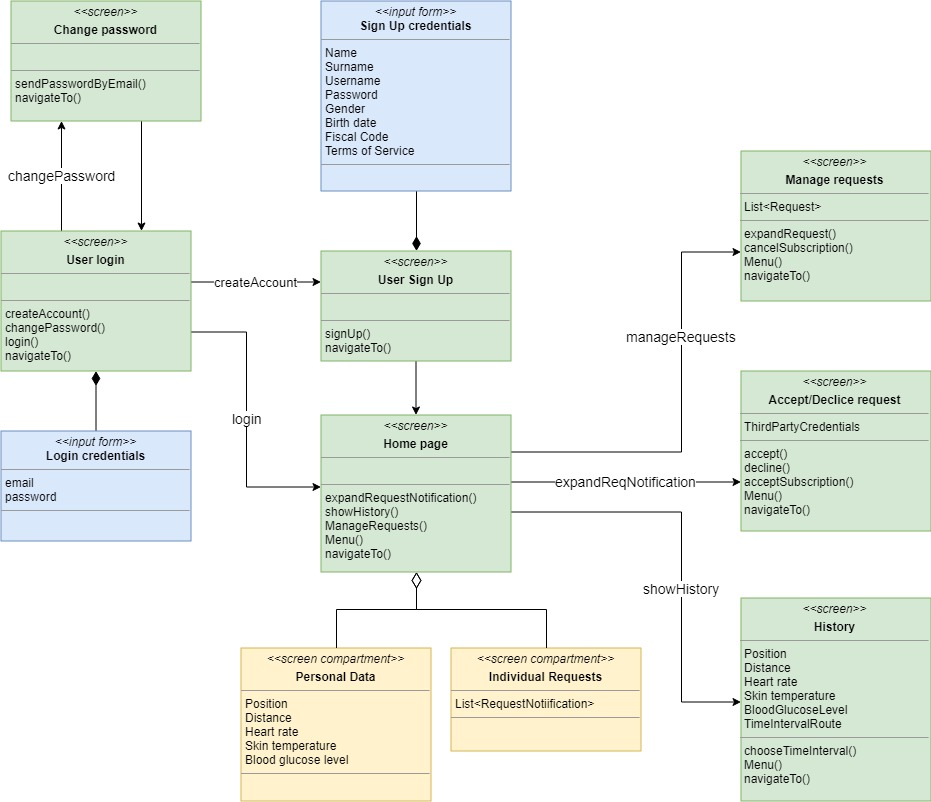
\includegraphics[width=300pt]{images/UX/UX_Diagram1.jpg}
    \caption{Data4Help - User experience}
    \label{UX1}
\end{figure}
\clearpage
The second diagram describes the experience of the third party through the mobile application(or maybe also through the Web application). The first page that he/she has to face is obviously the login screen, from which he/she can reach the Registration or the Home pages. Finally, from this last screen the third party can reach the Create Group Request, Create Individual Request and the Data pages.
\begin{figure}[ht]
    \centering
    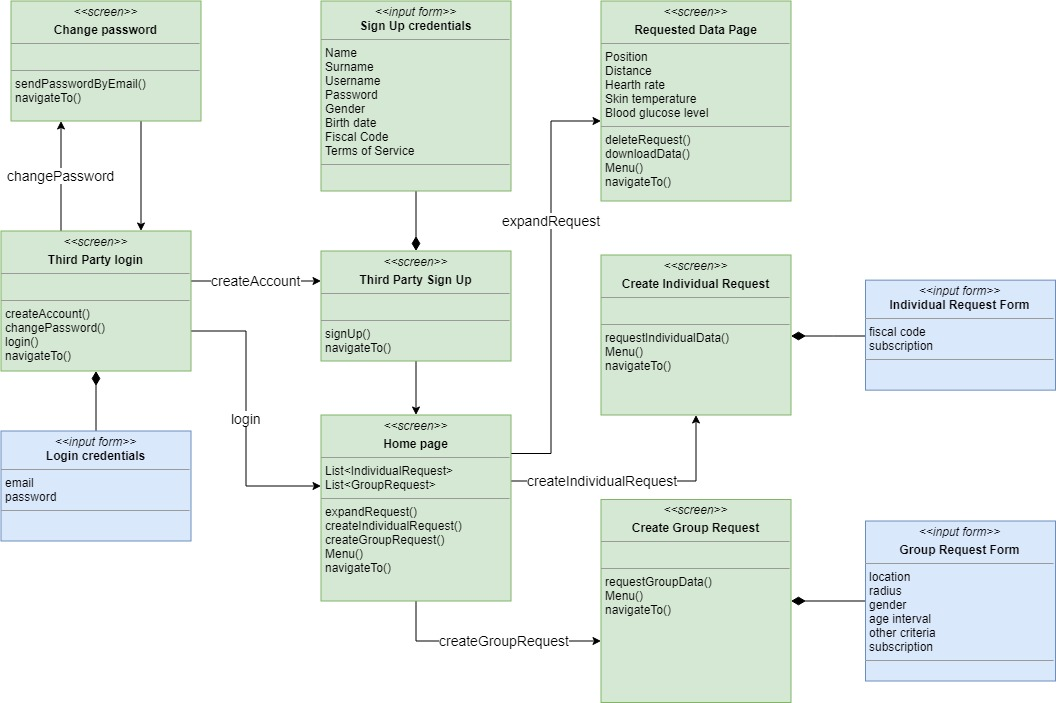
\includegraphics[width=300pt]{images/UX/UX_Diagram2.jpg}
    \caption{Data4Help - third party experience}
    \label{UX2}
\end{figure}
\clearpage
This last diagram illustrates the experience of a User through the AutomatedSOS mobile application(or maybe also through wearable application). As in the other applications, the first page that the user has to face is the Login page, followed by the Registration or Home pages. The last available page of this application is the Emergency screen and it can be reach from the Home page by clicking on its button, when an emergency is detected.
\begin{figure}[ht]
    \centering
    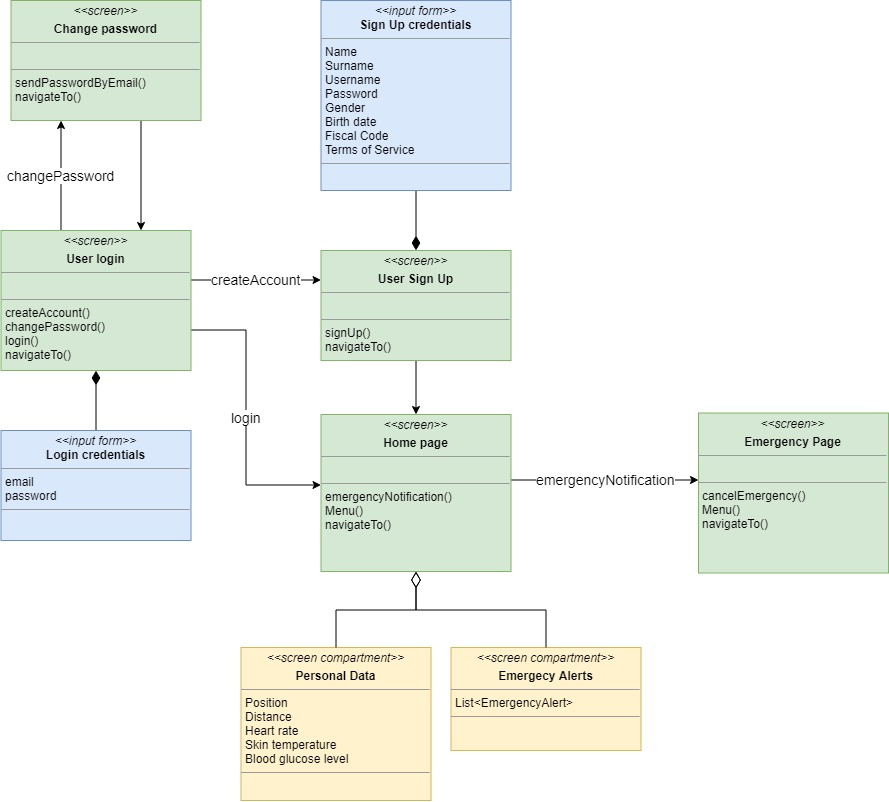
\includegraphics[width=300pt]{images/UX/UX_Diagram3.jpg}
    \caption{AutomatedSOS - User experience}
    \label{UX3}
\end{figure}
\clearpage

\section{Boundary Control Entity Diagrams}
In the last section of the chapter focused on the User Interfaces we wants to reach a further level of detail.\\
We showed all the available pages of our applications-to-be and how the user or the third party can navigate through them.\\
Here we want to illustrate how the interactions of a User/Third Party with respective applications are managed by the \say{Controller} and their effects on the \say{Model}.
In the following diagrams we refer to the Model-View-Controller design pattern, which guarantee the correct separation between the presentation of the application and its core logic.\\
The entities on the left are intended as part of the View of our applications-to be, the entities on the right are part of the Model and, for last, the ones at the center represent the Controller.

\begin{figure}[ht]
    \centering
    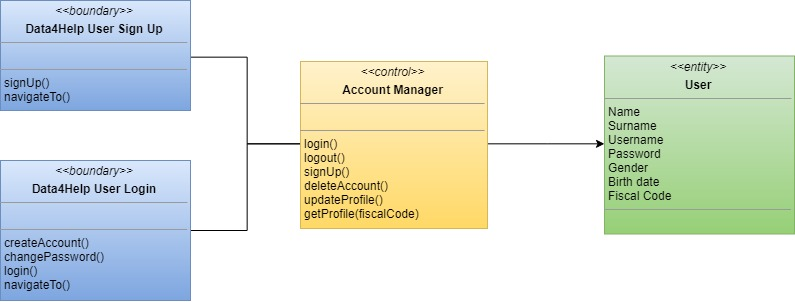
\includegraphics[width=300pt]{images/BCE/BCE_Diagrams1.jpg}
    \caption{User registration and login to Data4Help application.}
    \label{BCE1}
\end{figure}
\begin{figure}[ht]
    \centering
    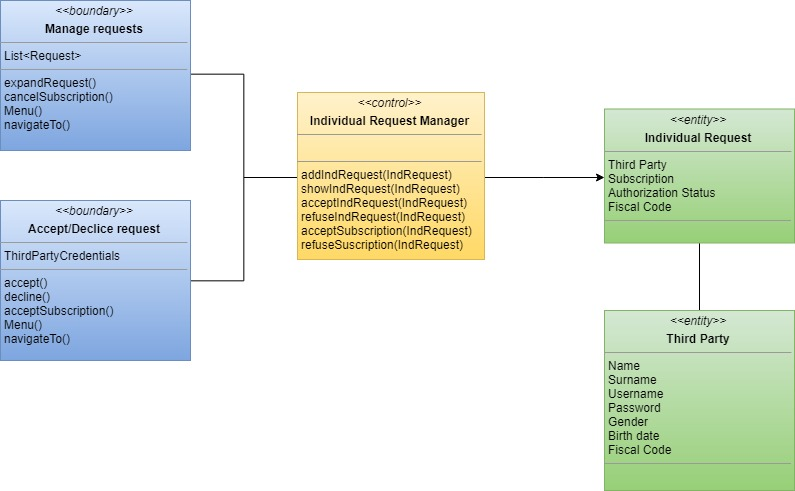
\includegraphics[width=300pt]{images/BCE/BCE_Diagrams2.jpg}
    \caption{The user respond to a request and manages previous requests.}
    \label{BCE2}
\end{figure}
\begin{figure}[ht]
    \centering
    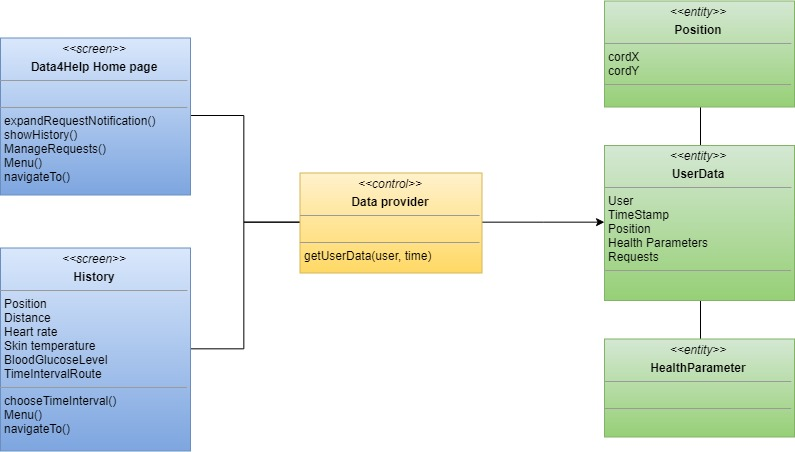
\includegraphics[width=300pt]{images/BCE/BCE_Diagrams3.jpg}
    \caption{The user accesses current or historical personal data.}
    \label{BCE3}
\end{figure}
\begin{figure}[ht]
    \centering
    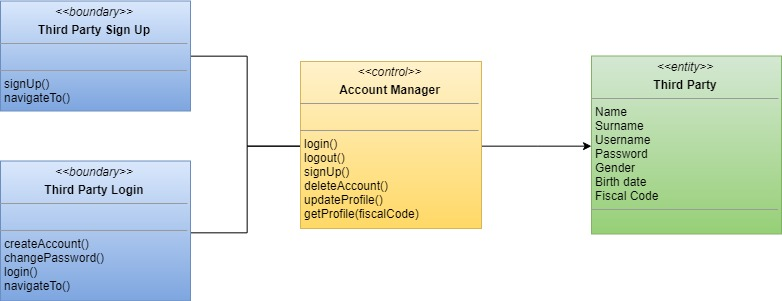
\includegraphics[width=300pt]{images/BCE/BCE_Diagrams4.jpg}
    \caption{Third party registration and login to the Data4Help application.}
    \label{BCE4}
\end{figure}
\begin{figure}[ht]
    \centering
    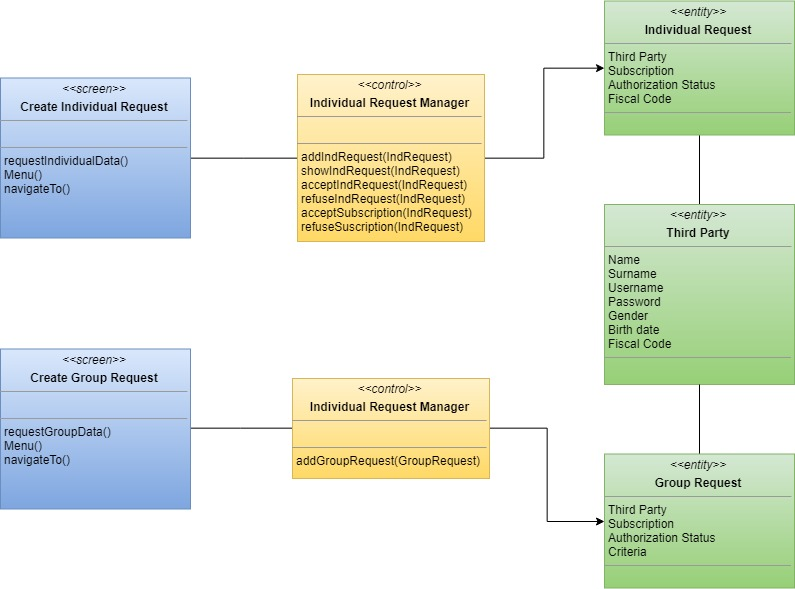
\includegraphics[width=300pt]{images/BCE/BCE_Diagrams5.jpg}
    \caption{The third party creates an individual or group request.}
    \label{BCE5}
\end{figure}
\begin{figure}[ht]
    \centering
    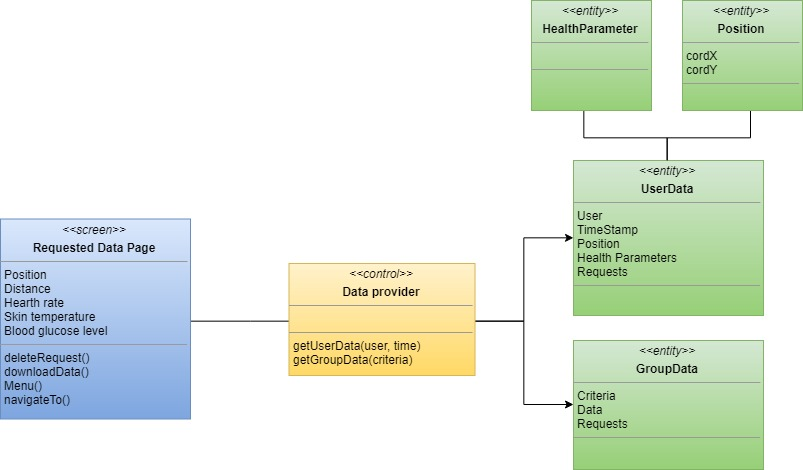
\includegraphics[width=295pt]{images/BCE/BCE_Diagrams6.jpg}
    \caption{The third party obtains the requested data.}
    \label{BCE6}
\end{figure}
\begin{figure}[ht]
    \centering
    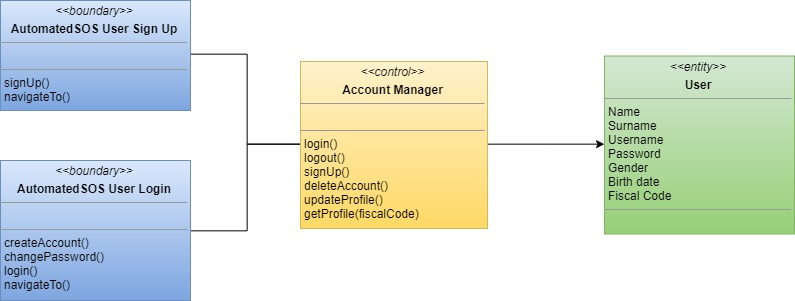
\includegraphics[width=295pt]{images/BCE/BCE_Diagrams7.jpg}
    \caption{User registration and login to AutomatedSOS application.}
    \label{BCE7}
\end{figure}
\begin{figure}[ht]
    \centering
    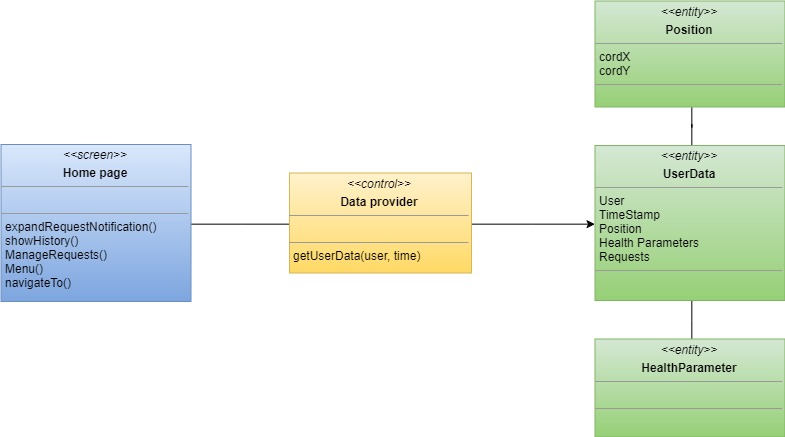
\includegraphics[width=295pt]{images/BCE/BCE_Diagrams8.jpg}
    \caption{The user accesses current personal data.}
    \label{BCE8}
\end{figure}
\begin{figure}[ht]
    \centering
    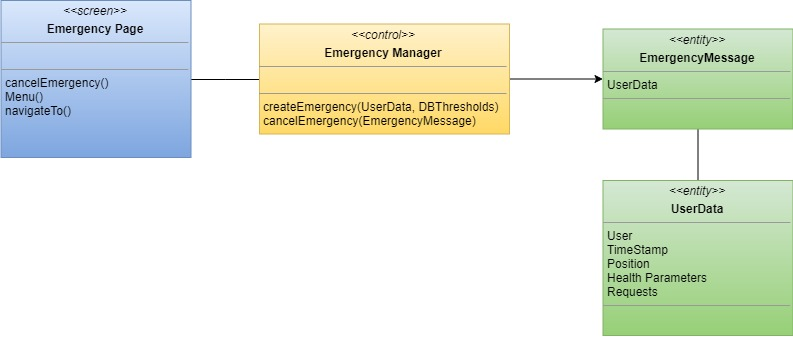
\includegraphics[width=300pt]{images/BCE/BCE_Diagrams9.jpg}
    \caption{Emergency Page activated in case of a health crisis.}
    \label{BCE9}
\end{figure}